\documentclass{article}

\usepackage{microtype}
\usepackage{graphicx}
\usepackage{subfigure}
\usepackage{booktabs}
\usepackage{hyperref}
\usepackage{multirow}

\newcommand{\theHalgorithm}{\arabic{algorithm}}

\usepackage[accepted]{icml2025}

\usepackage{amsmath}
\usepackage{amssymb}
\usepackage{mathtools}
\usepackage{amsthm}
\usepackage{xcolor}
\usepackage{colortbl}
\usepackage{float}

\usepackage[capitalize,noabbrev]{cleveref}

\icmltitlerunning{HW8: Discovering Carry Propagation Circuits}

\begin{document}

\twocolumn[
\icmltitle{Discovering Carry Propagation Circuits in a Small Addition Transformer \\
           \vspace{0.15in}
           \textnormal{\normalsize Homework 8 --- Research in LLMs, HSE $\times$ Central University}}

\begin{center}
    \textbf{Ivan A. Novosad} \\
    \texttt{inovosad@hse.ru} \\
\end{center}

\vskip 0.3in
]

\section{Introduction and Setup}
\label{sec:intro}

Autoregressive transformers predict digits left-to-right, but carry propagation in addition is fundamentally right-to-left: whether the hundreds digit is 4 or 5 depends on the ones and tens columns, which the model has not yet output.
The model must therefore \emph{anticipate} carries from lower-significance digits.
Can I find a dedicated carry circuit, or is carry an emergent effect of distributed computation?

I study a 2-layer, 3-head transformer (${\sim}$398K parameters) trained on 3-digit addition with character-level tokenization in standard MSB-first digit order.
Inputs are zero-padded (\texttt{012+034=0046$\langle$EOS$\rangle$}, 13 tokens).
Training uses carry-enriched data: balanced chain-length sampling ensures ${\sim}$25\% cascade cases.
The model is deliberately trained on CPU---interpretability, not scale.

Character-level tokenization is critical for the circuit structure I study.
Models with multi-digit tokenizers (e.g., GPT-2, which encodes integers 0--512 as single tokens) perform addition via lookup-table heuristics rather than algorithmic carry propagation~\citep{nikankin2024arithmetic}.
Character-level tokenization forces the model to handle carry digit-by-digit: each output token depends on the corresponding input digit pair plus any incoming carry, producing the modular per-position circuits I aim to discover.
This is why I train a custom model rather than analyzing a pre-trained LLM.

Table~\ref{tab:accuracy} shows the final validation accuracy.
The model achieves perfect accuracy on no-carry (BA) and single-carry (MC1) cases, but only 91.3\% on full cascades (S3), indicating the model has not fully solved cascading carries.
Failures concentrate in the hundreds digit (92.5\% for S3), exactly where cascading carry resolution is hardest.

Figure~\ref{fig:training} shows training dynamics.
Learning is phased: BA converges first (by step 2000), then MC1 (step 4000), then US9/S3 (step 8000+), consistent with Quirke \& Barez's~\cite{quirke2024understanding} finding that carry-related skills emerge after base addition is learned.

\begin{table}[t]
\caption{Final validation accuracy (step 11500). Ones and tens digits are perfectly predicted across all categories; errors concentrate in hundreds and overflow digits for cascade cases.}
\label{tab:accuracy}
\centering
\small
\begin{tabular}{lcccc}
\toprule
& \textbf{Overflow} & \textbf{Hundreds} & \textbf{Tens} & \textbf{Ones} \\
\midrule
BA   & 100.0 & 100.0 & 100.0 & 100.0 \\
MC1  & 100.0 & 100.0 & 100.0 & 100.0 \\
US9  & 99.4  & 96.8  & 100.0 & 100.0 \\
S3   & 98.5  & 92.5  & 100.0 & 100.0 \\
\midrule
Overall & \multicolumn{4}{c}{96.97\% (uniform test set)} \\
\bottomrule
\end{tabular}
\end{table}

\begin{figure*}[t]
\centering
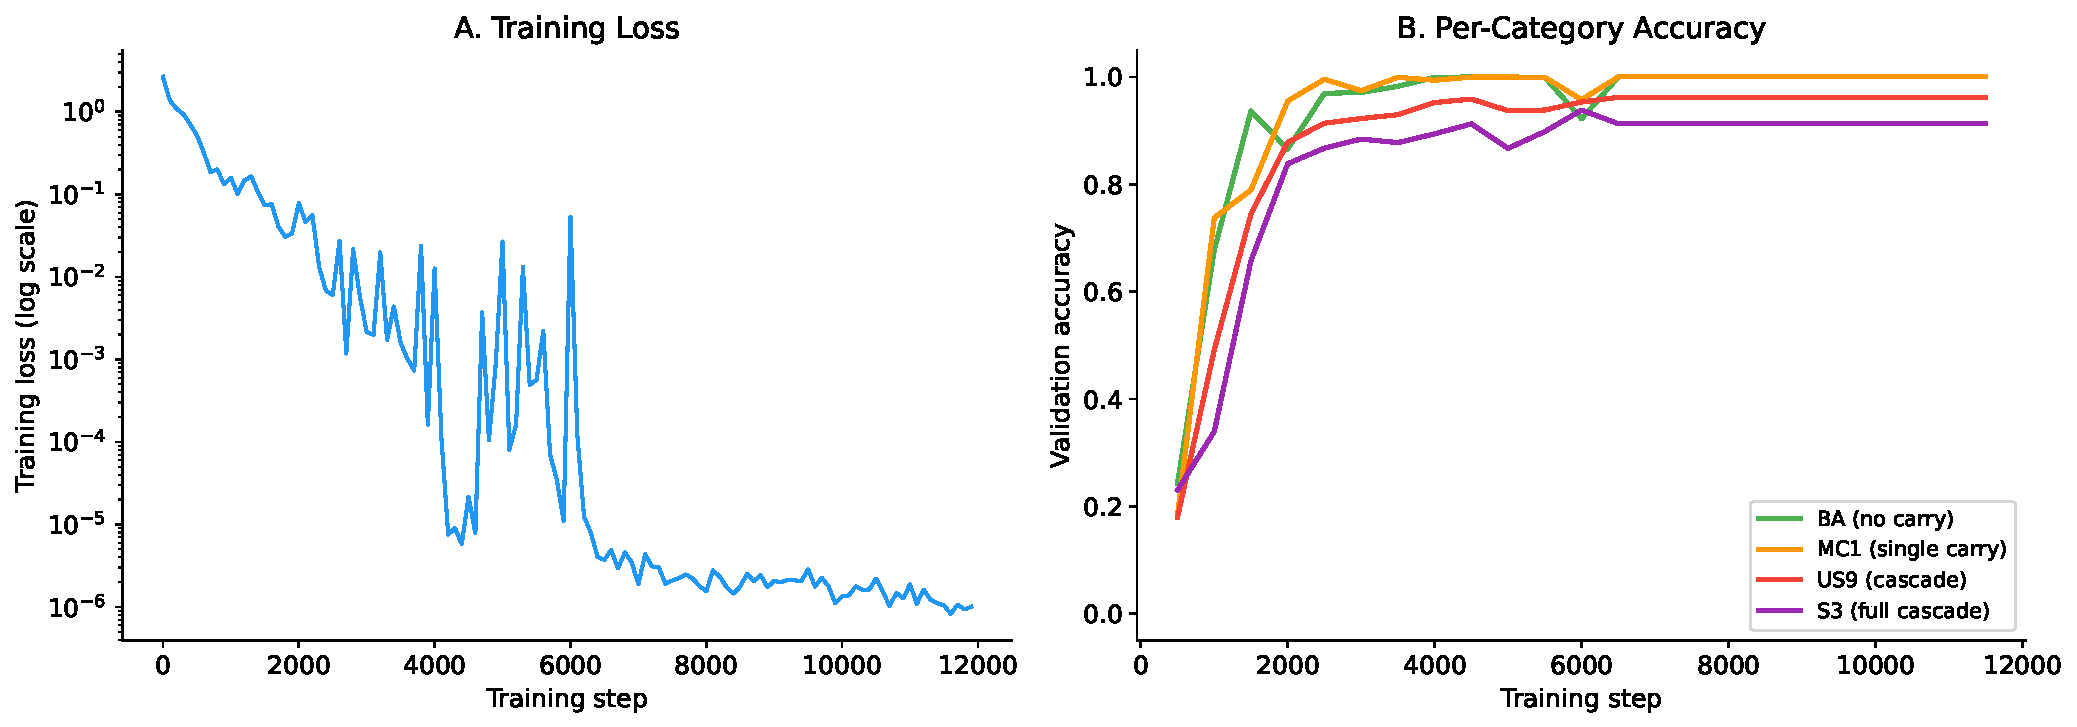
\includegraphics[width=\textwidth]{figures/fig1_training.pdf}
\caption{Training dynamics. \textbf{A:} Training loss decreases monotonically over 12K steps. \textbf{B:} Per-category accuracy shows phased learning---BA converges first, followed by MC1, then US9 and S3 (cascading carries). This ordering matches the literature: carry skills build on base addition.}
\label{fig:training}
\end{figure*}

\section{Experimental Methodology}
\label{sec:methods}

\subsection{Counterfactual Pair Design}

I construct three types of counterfactual pairs (500 pairs each) to isolate specific carry effects:

\textbf{Type~A (single carry isolation).}
The clean input has a carry at exactly one position; the corrupted input does not.
Only one digit of operand~$a$ is changed.
Example for ones carry: clean $25 + 759 = 784$ (carry at ones: $5+9=14$) vs.\ corrupted $20 + 759 = 779$ (no carry: $0+9=9$).
The answer differs at the tens digit (8 vs 7), isolating the carry's downstream effect.
I generate subtypes for ones, tens, and hundreds positions.

\textbf{Type~B (cascade isolation).}
Both inputs have a carry at the ones position.
The clean input has a tens digit-sum of exactly 9, so the ones carry cascades through; the corrupted input has a tens digit-sum $\leq 7$, so the carry is absorbed.
This isolates the cascade mechanism from the initial carry.

\textbf{Type~C (confound control).}
Clean and corrupted produce the \emph{same} ones answer digit but differ in whether a carry occurs (e.g., $5+9=14$ vs.\ $4+0=4$).
This ensures that any observed patching effect reflects carry information rather than differences in the ones output digit.

\subsection{Patching Methodology}

The idea behind denoising activation patching is simple: run the model on the wrong input, then surgically restore one component's activation from the correct input. If the output flips back to correct, that component was carrying the relevant information.

I could also run noising (patch corrupted activations into a clean run) to test necessity directly, but started with denoising because it gives a cleaner signal for exploration --- if restoring one component's activation is enough to recover the output, that component carries the relevant information. Section~4 uses mean ablation, which is effectively noising, to validate.

The primary metric is \textbf{logit difference recovery}.
For each pair, I compute $\text{LD} = \text{logit}(y_\text{clean}) - \text{logit}(y_\text{corrupted})$ at the primary answer position.
Recovery is the fraction of the clean--corrupted gap restored by patching:
\begin{equation}
\text{Recovery} = \frac{\text{LD}_\text{patched} - \text{LD}_\text{corrupted}}{\text{LD}_\text{clean} - \text{LD}_\text{corrupted}}
\label{eq:recovery}
\end{equation}
Logit difference is the appropriate metric because residual stream additions are linear in logit space~\cite{zhang2024best}.

For head-level analysis, I also use the \textbf{Stolfo symmetric indirect effect}~\cite{stolfo2023mechanistic}:
\begin{equation}
\text{IE} = \frac{1}{2}\!\left(\frac{P^*(r') - P(r')}{P(r')} + \frac{P(r) - P^*(r)}{P^*(r)}\right)
\label{eq:ie}
\end{equation}
where $P$ are probabilities from the base run on prompt~$p$, and $P^*$ are probabilities when activations at the mediator are replaced with those from prompt~$p'$.
In practice, I use logit difference recovery (Eq.~\ref{eq:recovery}) as the primary metric because logit differences are additive in the residual stream.
I report Stolfo IE as a secondary check; denominators are clamped to $10^{-10}$ for numerical stability.

\subsection{Coarse-to-Fine Analysis}

I work coarse-to-fine:
(1) \textbf{Residual stream patching} identifies \emph{where} (which token positions and layers) carry information flows;
(2) \textbf{Component-level patching} determines \emph{what type} of component (attention vs.\ MLP) mediates carry at each layer;
(3) \textbf{Head-level IE sweep} pinpoints \emph{which specific heads} are carry-critical;
(4) \textbf{Circuit validation} tests whether the identified components form a coherent, necessary, and sufficient circuit.

\section{Where is Carry Computation?}
\label{sec:results}

\subsection{Residual Stream Patching}

If carry computation follows \citet{quirke2024understanding}'s two-stage pattern, carry information should originate at operand digit positions and arrive at answer positions by Layer~1.

Figure~\ref{fig:residual} shows the residual stream patching heatmap for Type~A pairs.
Carry information concentrates sharply: for ones carry, the signal appears at position $a_O$ (the ones digit of operand~$a$) in layer~0, then at position $s_H$ (the hundreds answer position) by layer~1.
Tens carry follows the same pattern shifted: position $a_T$ at layer~0, position $s_H$ at layer~1.
Hundreds carry information originates at position $a_H$ with strong recovery (0.92) already between layers 0 and 1.

Carry information is picked up from operand digit positions, then routed to answer positions---matching the two-stage pattern from \citet{quirke2024understanding}.

\begin{figure*}[t]
\centering
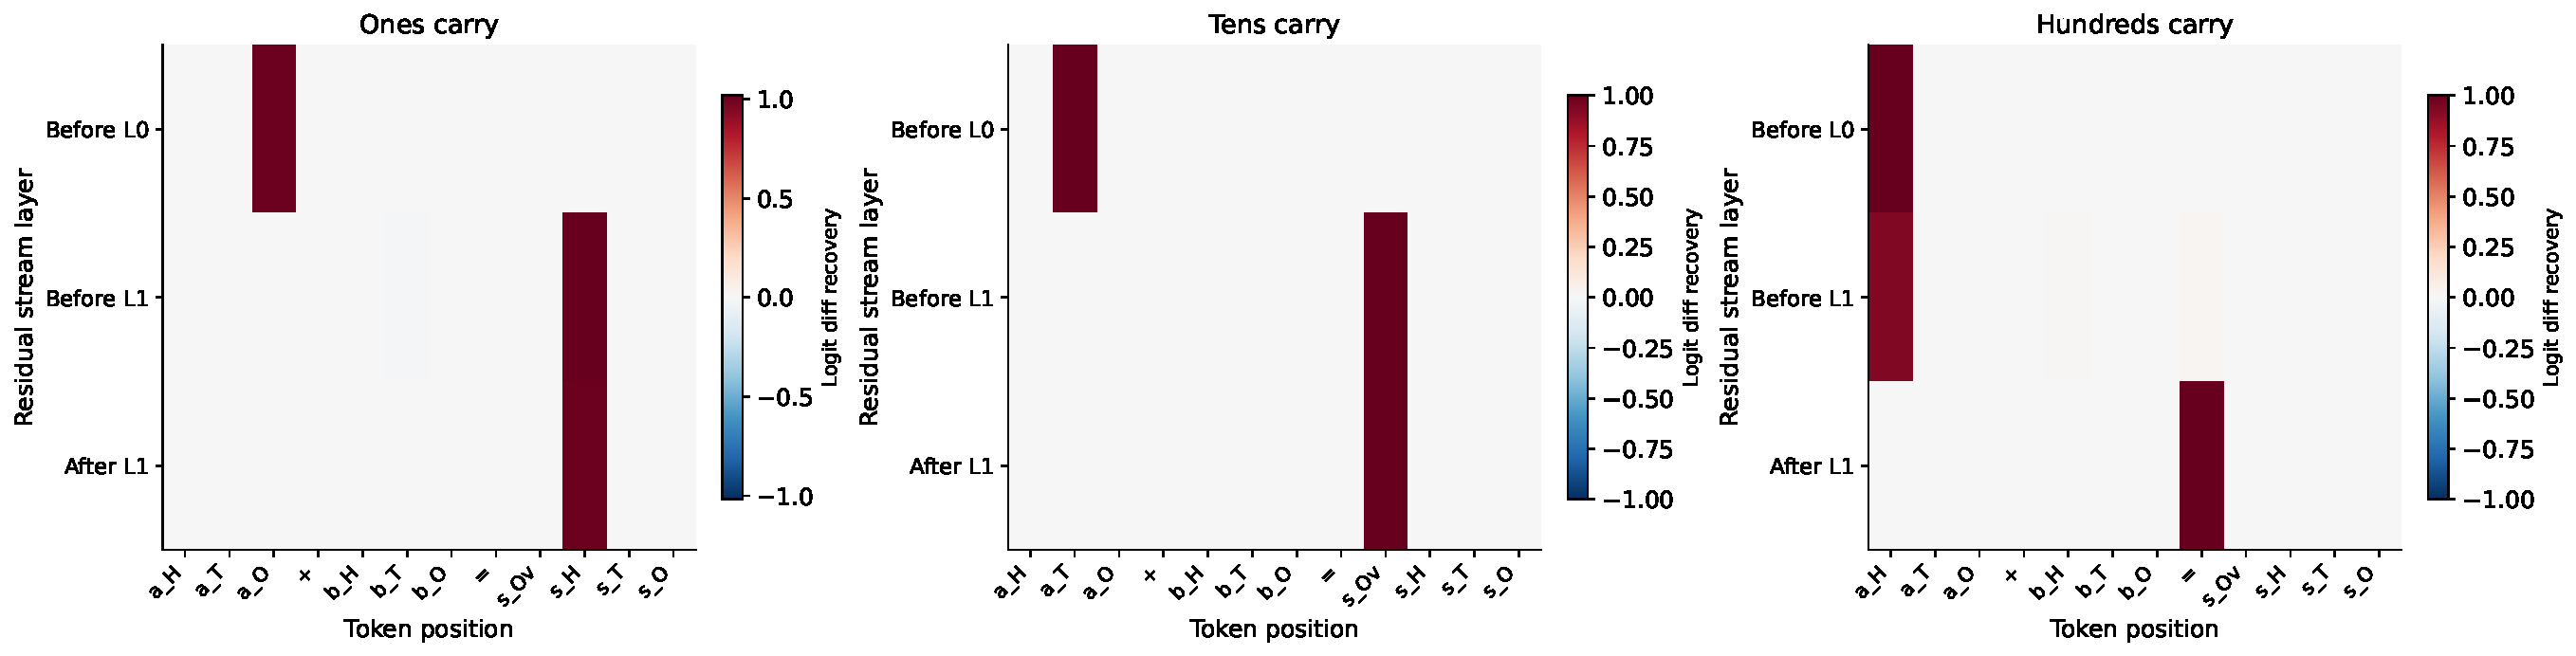
\includegraphics[width=\textwidth]{figures/fig2_residual.pdf}
\caption{Residual stream patching (logit difference recovery). Each panel shows one carry type. Carry information originates at the operand digit that triggers the carry and arrives at the answer position where the carry modifies the output. Recovery of 1.0 means full restoration of the clean model's logit difference.}
\label{fig:residual}
\end{figure*}

\subsection{Component-Level Patching}

Figure~\ref{fig:component} breaks down recovery by component type.
For ones and tens carry, \textbf{L0-Attn} dominates at the primary answer position (recovery ${\approx}1.0$), with L0-MLP and L1-MLP providing secondary contributions ($0.97$ and $0.99$ respectively).
For hundreds carry, \textbf{L1-Attn} leads (recovery $0.98$ at the overflow position), with L0-MLP at $0.83$.

L0 attention detects local carries at the ones and tens positions. For hundreds carry, which requires integrating information from lower positions, L1 attention takes over.

\begin{figure*}[t]
\centering
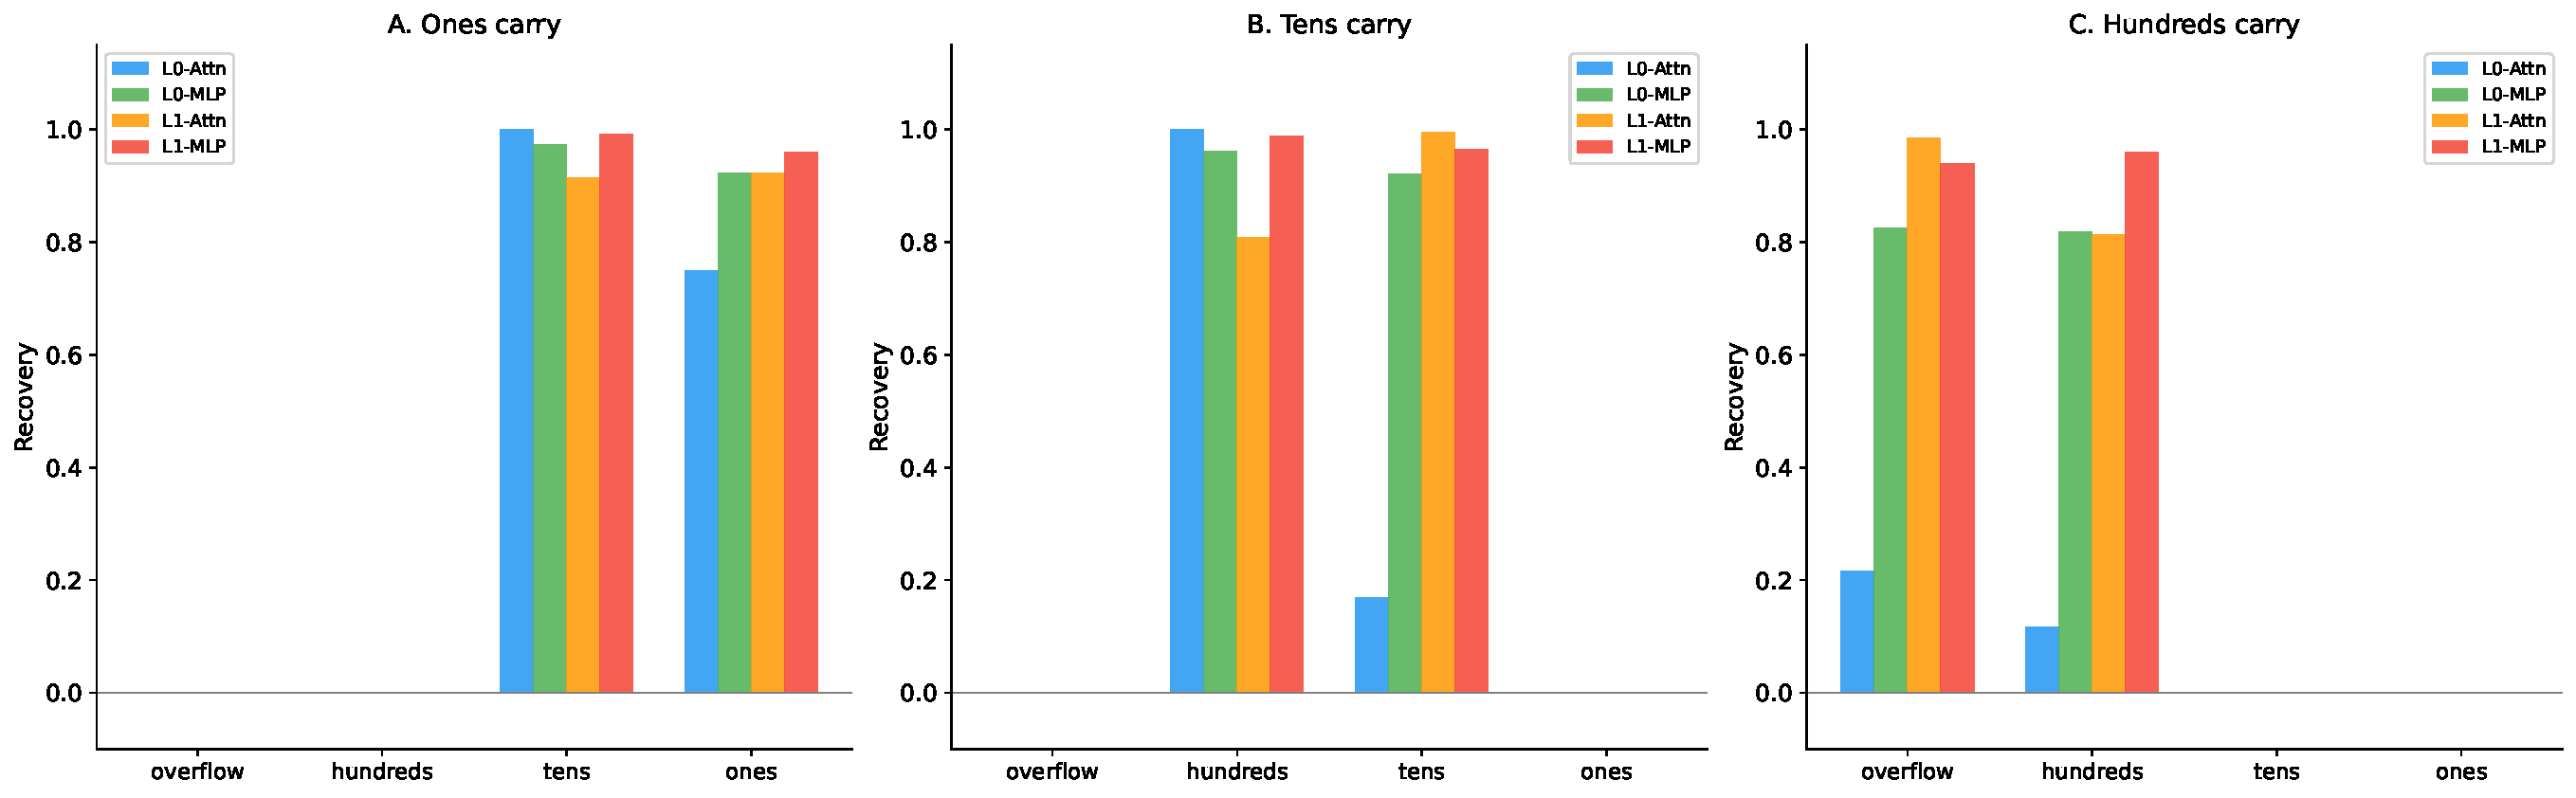
\includegraphics[width=\textwidth]{figures/fig7_component.pdf}
\caption{Component-level patching recovery by answer position. L0-Attn dominates for ones and tens carry; L1-Attn leads for hundreds carry, suggesting a two-stage detection--composition pipeline.}
\label{fig:component}
\end{figure*}

\subsection{Head-Level IE Sweep}

If the two-stage pattern from Section~3.2 holds at head level, I expect Layer~0 heads to detect local carries and Layer~1 heads to handle cross-position composition.

Figure~\ref{fig:head_ie} presents the main result: head-level indirect effect for all six heads across four carry types.
Three heads emerge as carry-critical.
L0H2 is the ones-carry head: IE = 0.98 at the tens position for Type~A ones pairs, and essentially zero for tens or hundreds carry.
L0H1 handles tens carry and cascades --- IE = 0.995 for tens pairs, 0.997 for cascade pairs, both at the hundreds position.
L1H2 plays a different role: it shows up everywhere, with IE between 0.79 and 0.92 across all carry types. This consistency suggests it integrates carry signals from Layer~0 rather than detecting carries itself.

The ``Type~A: Hundreds'' panel uses a different colorbar scale (max ${\approx}0.33$ vs.\ ${\approx}1.0$ for other panels).
Hundreds carry is genuinely more distributed across heads, not just visually weaker.

\begin{figure*}[t]
\centering
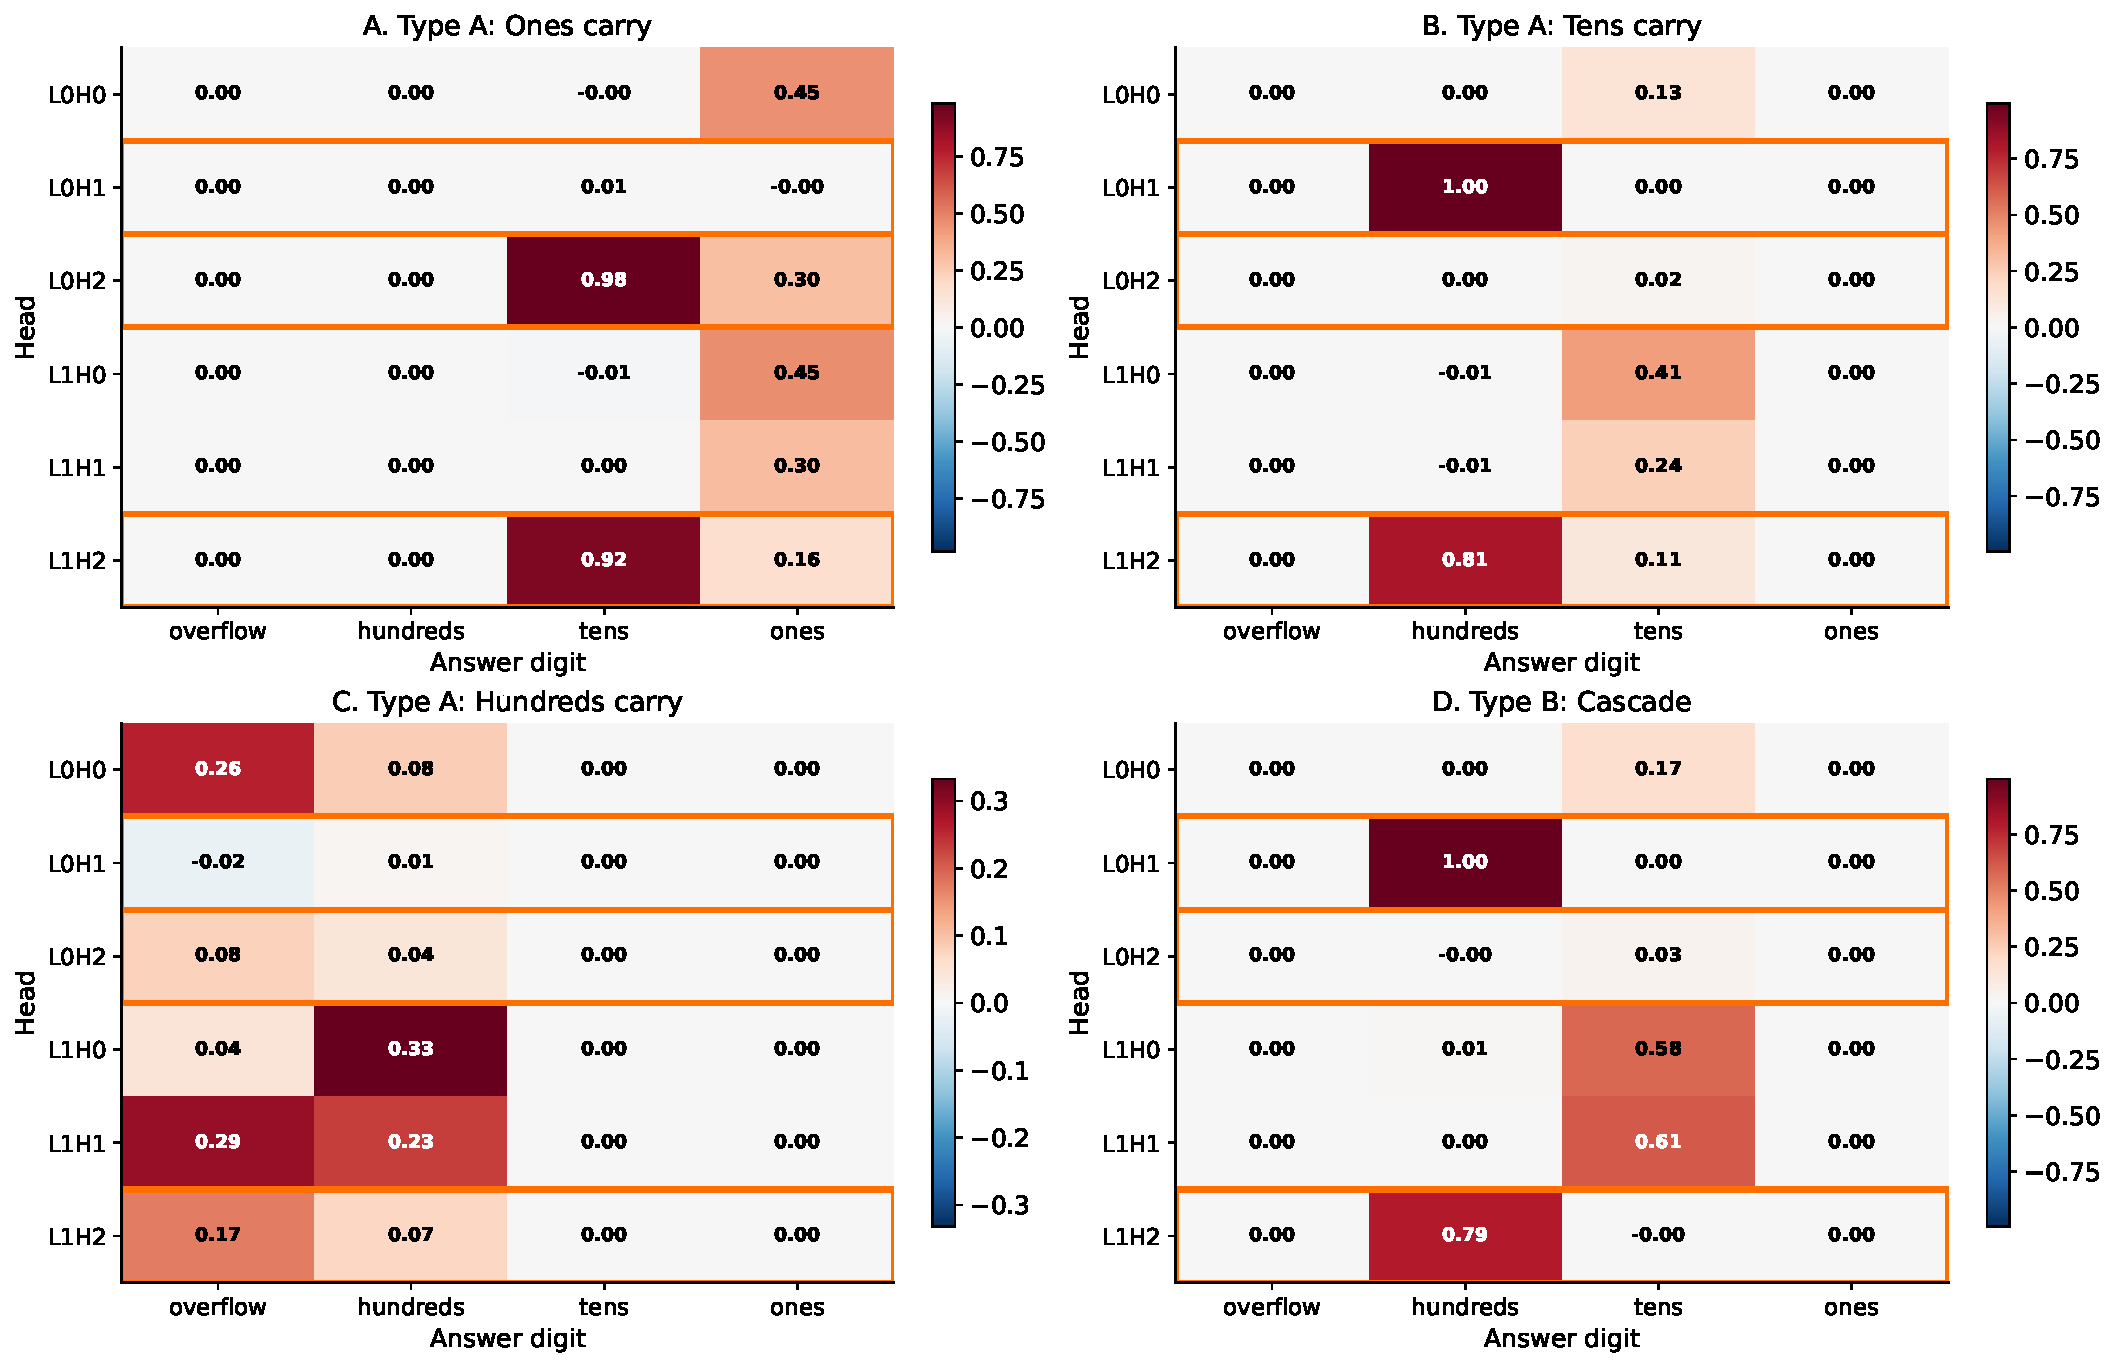
\includegraphics[width=\textwidth]{figures/fig3_head_ie.pdf}
\caption{Head-level indirect effect (main result). Rows are heads, columns are answer digit positions. L0H2 specializes in ones carry, L0H1 in tens/cascade carry, and L1H2 provides consistent secondary support. Orange borders highlight circuit components. Note: the hundreds carry panel has a different color scale (max ${\approx}0.33$), reflecting genuinely more distributed computation.}
\label{fig:head_ie}
\end{figure*}

\subsection{Attention Patterns}
\label{sec:attention}

Figure~\ref{fig:attention} shows attention patterns for a no-carry case (123+456=579) and a full cascade (999+001=1000).
I do \emph{not} observe the ``staircase'' attention pattern reported by Quirke \& Barez~\cite{quirke2024understanding}, where each answer position attends predominantly to corresponding operand digits in a regular diagonal pattern.

Several explanations are possible: (a) with only 3 digits, carry chains are short enough that heads can use more flexible attention without the rigid position-offset routing that produces staircases; (b) the model has 3 heads per layer (same as Quirke \& Barez's 5-digit models), but the shorter sequences give each head less need to specialize into a strict positional role; (c) the model may have found an alternative algorithm that achieves carry propagation without staircase structure.

\begin{figure*}[t]
\centering
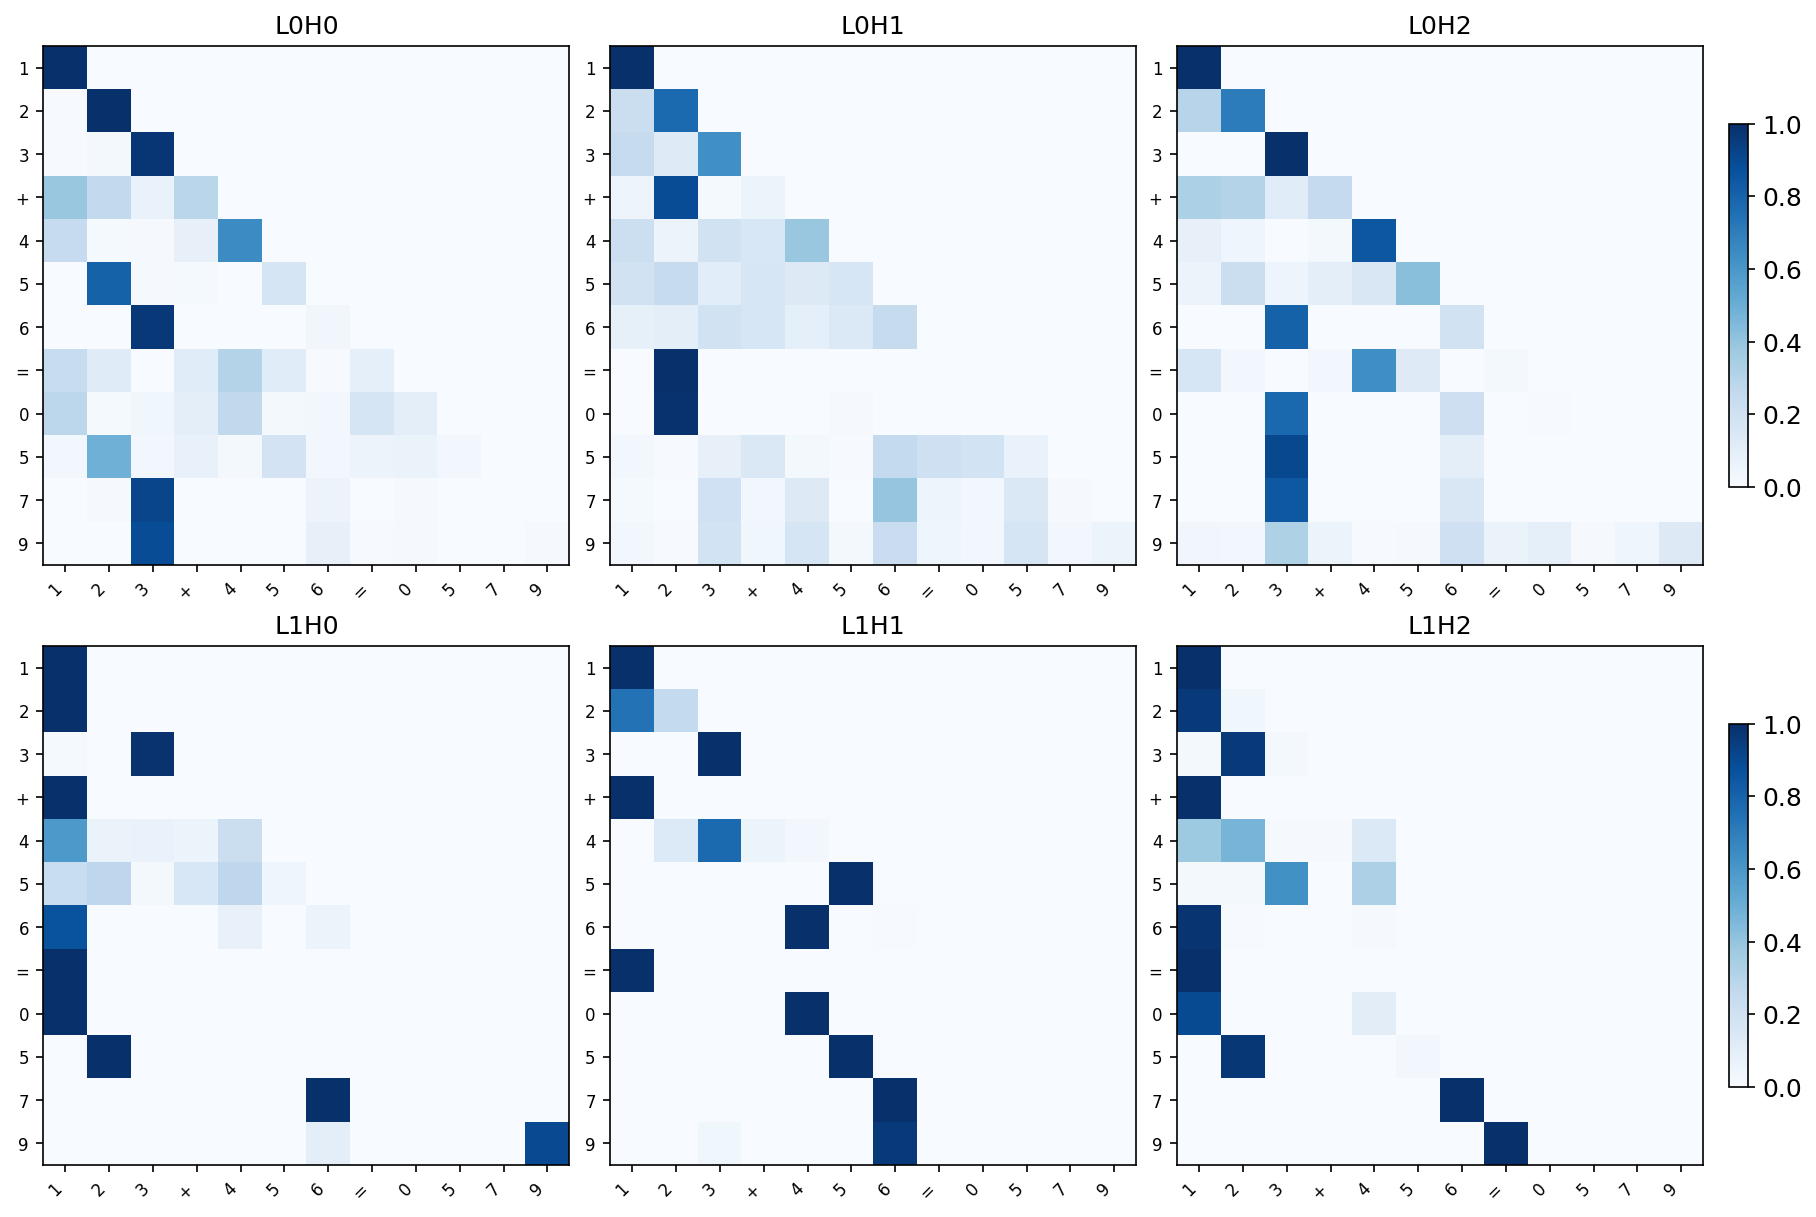
\includegraphics[width=\textwidth]{figures/exp4_attention_patterns_no_carry.png}
\vspace{-8pt}
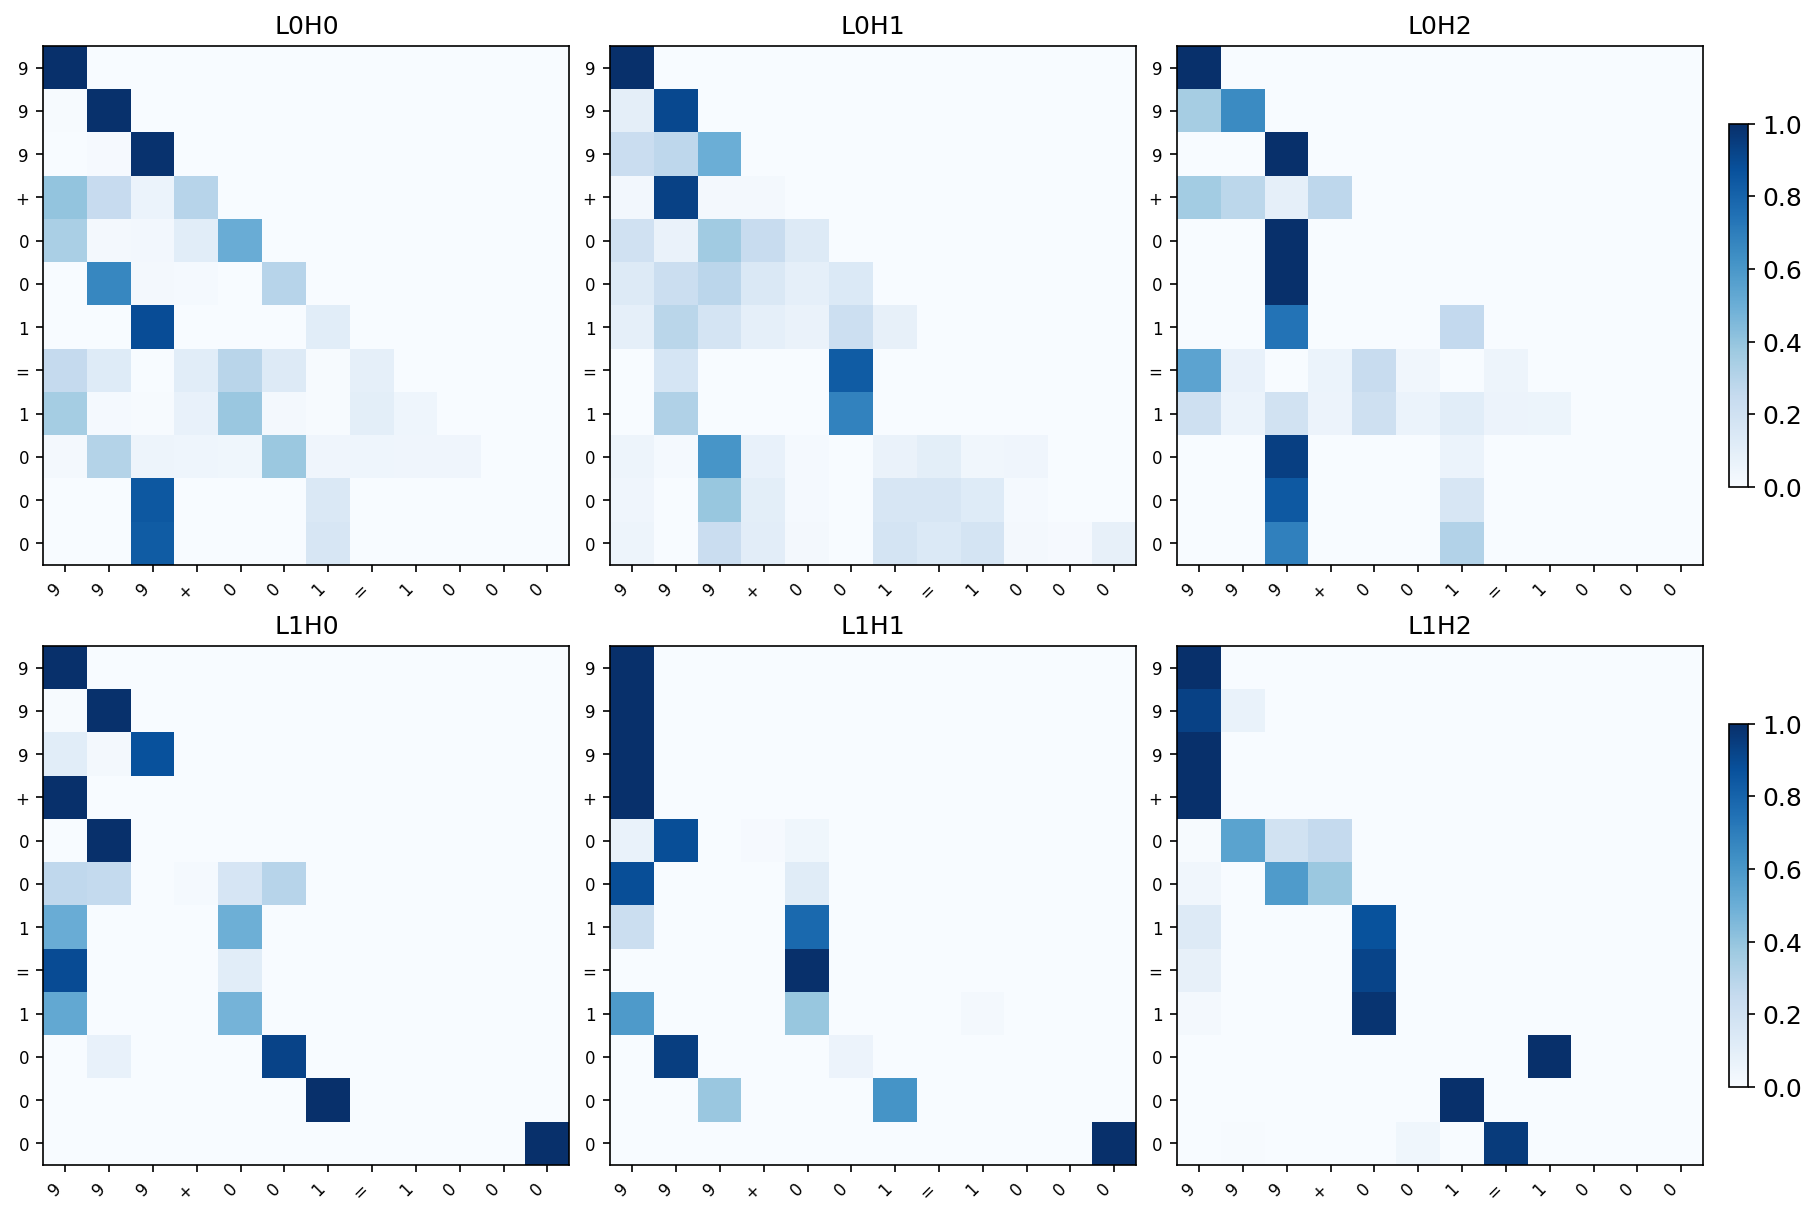
\includegraphics[width=\textwidth]{figures/exp4_attention_patterns_full_cascade.png}
\caption{Attention patterns for no-carry (top, 123+456=579) and full cascade (bottom, 999+001=1000). Each row is one layer, each column one head. The staircase pattern reported in the literature is absent. Instead, heads use flexible, context-dependent attention.}
\label{fig:attention}
\end{figure*}

\subsection{Direct Logit Attribution}

Table~\ref{tab:logit_attr} shows each head's mode output digit (via projection through the unembedding matrix) at each answer position, comparing carry vs.\ no-carry examples from Type~A ones pairs.
\textbf{Carry-sensitive positions} (where the mode digit changes between conditions) are highlighted.

L0H2 shifts from voting ``5'' (no-carry) to ``8'' (carry) at the tens position---directly reflecting the $+1$ carry adjustment.
L1H2 shifts from ``0'' to ``9'' at tens, and L1H0 changes its ones vote from ``5'' to ``1''.
In contrast, L0H1 votes identically in both conditions (always ``0'' at overflow/hundreds), confirming its role as a base-addition head whose output is \emph{read by} carry logic rather than directly encoding carry.

\begin{table}[t]
\caption{Direct logit attribution: mode digit voted by each head. Format: carry / no-carry. \colorbox{yellow!30}{Highlighted} cells differ between conditions (carry-sensitive).}
\label{tab:logit_attr}
\centering
\small
\setlength{\tabcolsep}{3pt}
\begin{tabular}{lcccc}
\toprule
& \textbf{Ovflw} & \textbf{Hund} & \textbf{Tens} & \textbf{Ones} \\
\midrule
L0H0 & 6/6 & 6/6 & 3/3 & \cellcolor{yellow!30}\textbf{1/2} \\
L0H1 & 0/0 & 0/0 & 7/7 & 7/7 \\
L0H2 & 5/5 & \cellcolor{yellow!30}\textbf{8/5} & \cellcolor{yellow!30}\textbf{8/5} & \cellcolor{yellow!30}\textbf{8/5} \\
L1H0 & 6/6 & 6/6 & 6/6 & \cellcolor{yellow!30}\textbf{1/5} \\
L1H1 & 3/3 & 6/6 & 3/3 & \cellcolor{yellow!30}\textbf{6/9} \\
L1H2 & 0/0 & 0/0 & \cellcolor{yellow!30}\textbf{9/0} & \cellcolor{yellow!30}\textbf{3/2} \\
\bottomrule
\end{tabular}
\end{table}

\subsection{What the Circuit Does}
\label{sec:mechanism}

Putting this together:
L0H1 computes digit-pair sums at adjacent positions and writes them to the residual stream; its output is carry-invariant (Table~\ref{tab:logit_attr}: identical votes in carry and no-carry conditions), making it the arithmetic substrate that carry logic reads from.
L0H2 detects ones-column carries: when $a_0 + b_0 \geq 10$, it shifts its logit vote from the no-carry answer digit to the carry-adjusted digit (Table~\ref{tab:logit_attr}: tens vote shifts from 5 to 8).
L1H2 integrates carry signals from Layer~0 across positions---its consistent IE across all carry types (0.79--0.92 in Figure~\ref{fig:head_ie}) indicates a general carry-composition role rather than position-specific detection.
L1-MLP combines these upstream signals into the final output logit.
In short: L0H1 provides digit-pair sums that L0H2 reads to detect carries. L1H2 then picks up these carry signals and composes them across positions, and L1-MLP produces the final corrected digit.

\section{Circuit Validation}
\label{sec:validation}

Based on the head-level IE results, I define the carry circuit as the set of components with max IE $> 0.3$ across any carry type, plus L1-MLP (expected from the literature to handle carry execution):
\textbf{L0H1, L0H2, L1H2, L1-MLP}---4 of 8 total components (50\% of the model).
Mean activations for ablation baselines are computed per-position over 2000 diverse examples.

\subsection{Necessity}

If these heads really are carry-specific, ablating them should break carry accuracy without touching non-carry performance.

Figure~\ref{fig:necessity} and Table~\ref{tab:necessity} show the results of single-component mean ablation on frozen test sets.
L0H1 ablation drops MC1 accuracy from 100\% to 5.2\% and S3 from 91.3\% to 0.4\%, while BA stays at 99.7\%. One head ablated, carry destroyed, non-carry intact --- this is the cleanest carry-specific signal in my experiments.

L0H2 ablation similarly damages carry categories (MC1 to 49.6\%, S3 to 50.3\%) while BA degrades less (to 94.4\%).
L1H2 ablation is less selective: BA drops to 67.6\%, and all carry categories fall to 38--47\%.

Group ablation of all circuit components yields near-zero accuracy across all categories, but so does ablating all non-circuit components.
This reflects the model's small size: both groups contain components essential for basic arithmetic, not just carry.

Table~\ref{tab:necessity} also reveals the shared arithmetic substrate.
Ablating L1-MLP or L0-MLP destroys all categories equally---including BA, which involves no carry at all.
These MLPs are essential for base arithmetic, not carry specifically.
L1H0 and L1H1 show similar patterns: their ablation causes near-total collapse across all categories, confirming they serve critical roles in the shared computation that carry heads depend on.

\begin{table}[t]
\caption{Necessity testing: accuracy after single-component ablation. Stars ($\star$) mark circuit components. L0H1 shows the strongest carry-specific effect.}
\label{tab:necessity}
\centering
\small
\begin{tabular}{lcccc}
\toprule
\textbf{Ablated} & \textbf{BA} & \textbf{MC1} & \textbf{US9} & \textbf{S3} \\
\midrule
(none) & 100.0 & 100.0 & 96.2 & 91.3 \\
\midrule
L0H1$^\star$ & 99.7 & 5.2 & 56.6 & 0.4 \\
L0H2$^\star$ & 94.4 & 49.6 & 43.2 & 50.3 \\
L1H2$^\star$ & 67.6 & 38.6 & 46.0 & 47.3 \\
L1-MLP$^\star$ & 0.0 & 0.0 & 0.0 & 0.0 \\
\midrule
L0H0 & 55.0 & 55.2 & 53.8 & 51.1 \\
L1H0 & 2.5 & 2.4 & 1.5 & 1.3 \\
L1H1 & 0.4 & 0.4 & 0.4 & 0.5 \\
L0-MLP & 0.0 & 0.3 & 0.2 & 0.3 \\
\bottomrule
\end{tabular}
\end{table}

\begin{figure}[t]
\centering
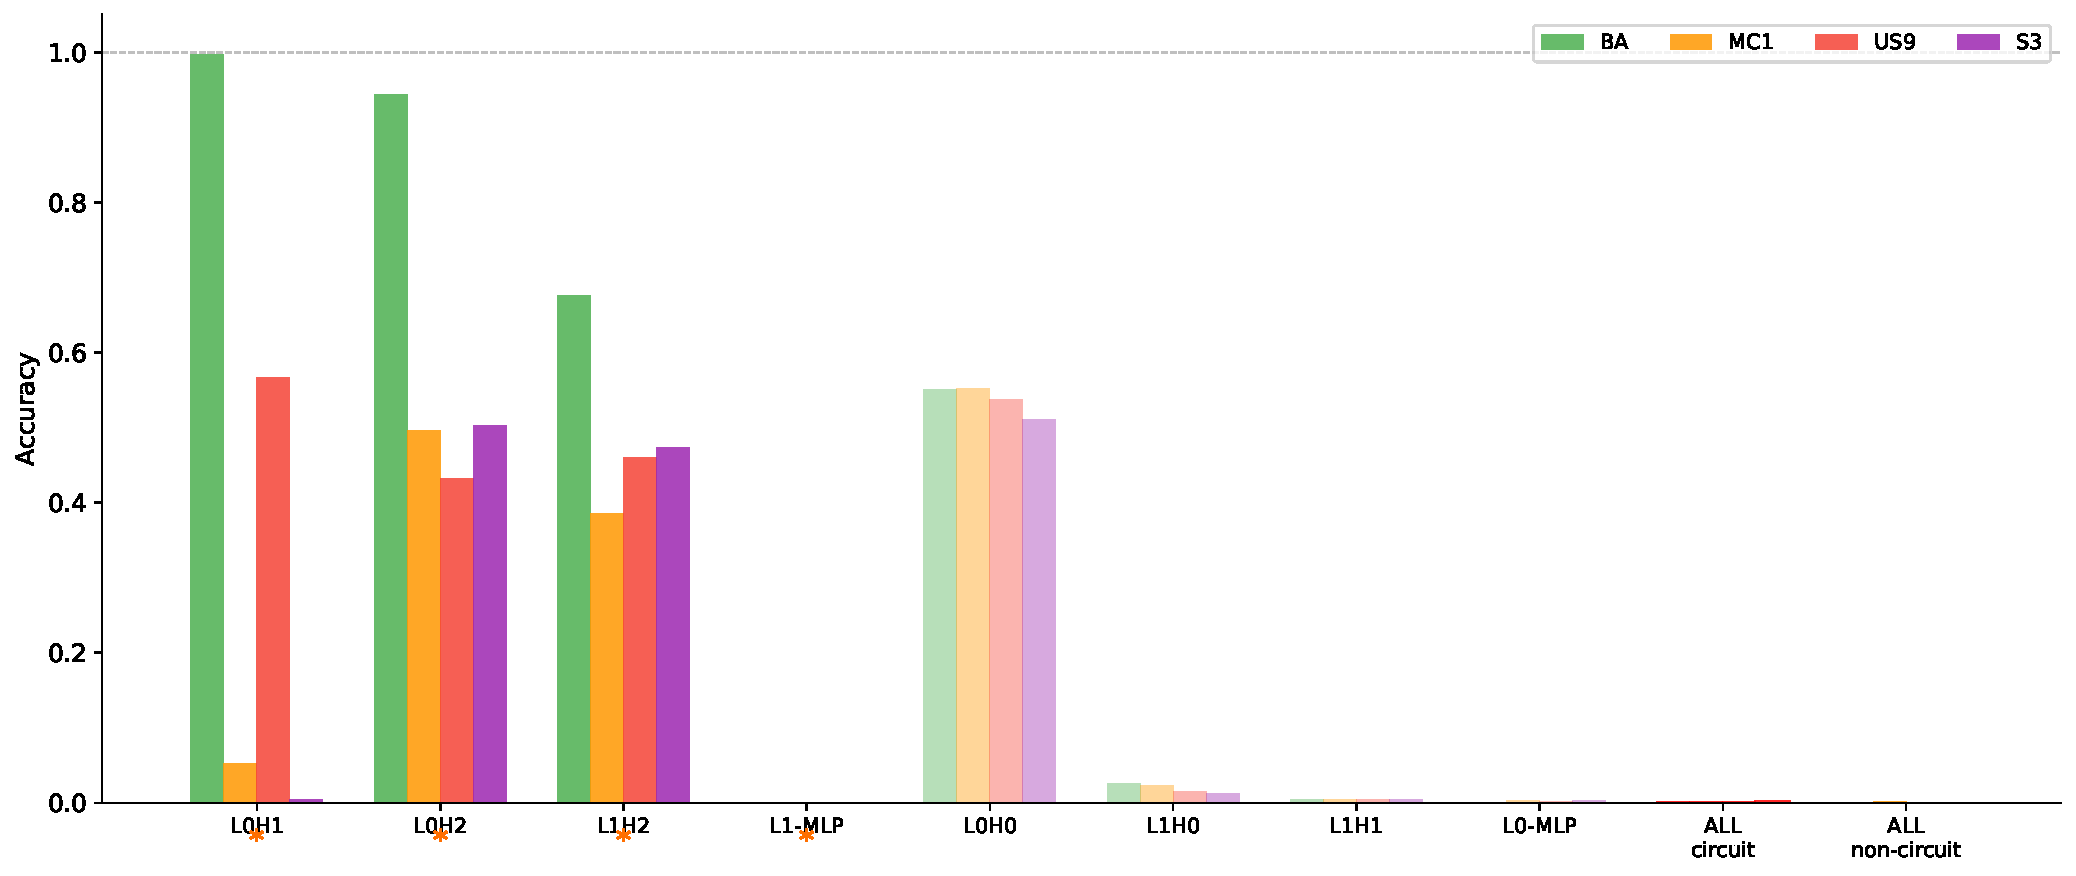
\includegraphics[width=\columnwidth]{figures/fig5_necessity.pdf}
\caption{Necessity testing: per-category accuracy after single-component ablation. Circuit components (marked with $\star$ in Table~\ref{tab:necessity}) show carry-specific degradation.}
\label{fig:necessity}
\end{figure}

\subsection{Sufficiency}

Figure~\ref{fig:sufficiency} shows what I did not expect: ablating all non-circuit components (running the model with \emph{only} the carry circuit) recovers essentially nothing---0.1\% of full model accuracy on BA, 0.2\% on MC1.
For comparison, the IOI circuit~\cite{wang2023interpretability} recovered 87--94\% of full model performance.

Carry detection requires knowing digit-pair sums ($a_n + b_n \geq 10$?), which are computed by the base-addition substrate---L0-MLP, L0H0, L1H0, L1H1.
The carry heads \emph{read} this information and add carry-specific adjustments.
Ablating everything except carry heads removes the substrate they read from.

The 100 random circuit baselines (same size: 4 components) show similarly near-zero recovery (mean 0.2\% $\pm$ 1.1\%), placing the circuit at the 73rd percentile---not significantly better than chance.
Not surprising --- half the model is not enough to do anything on its own.

The carry circuit is a \textbf{modifying overlay} --- necessary for carry, but dependent on the base-addition substrate it reads from.

\begin{figure}[t]
\centering
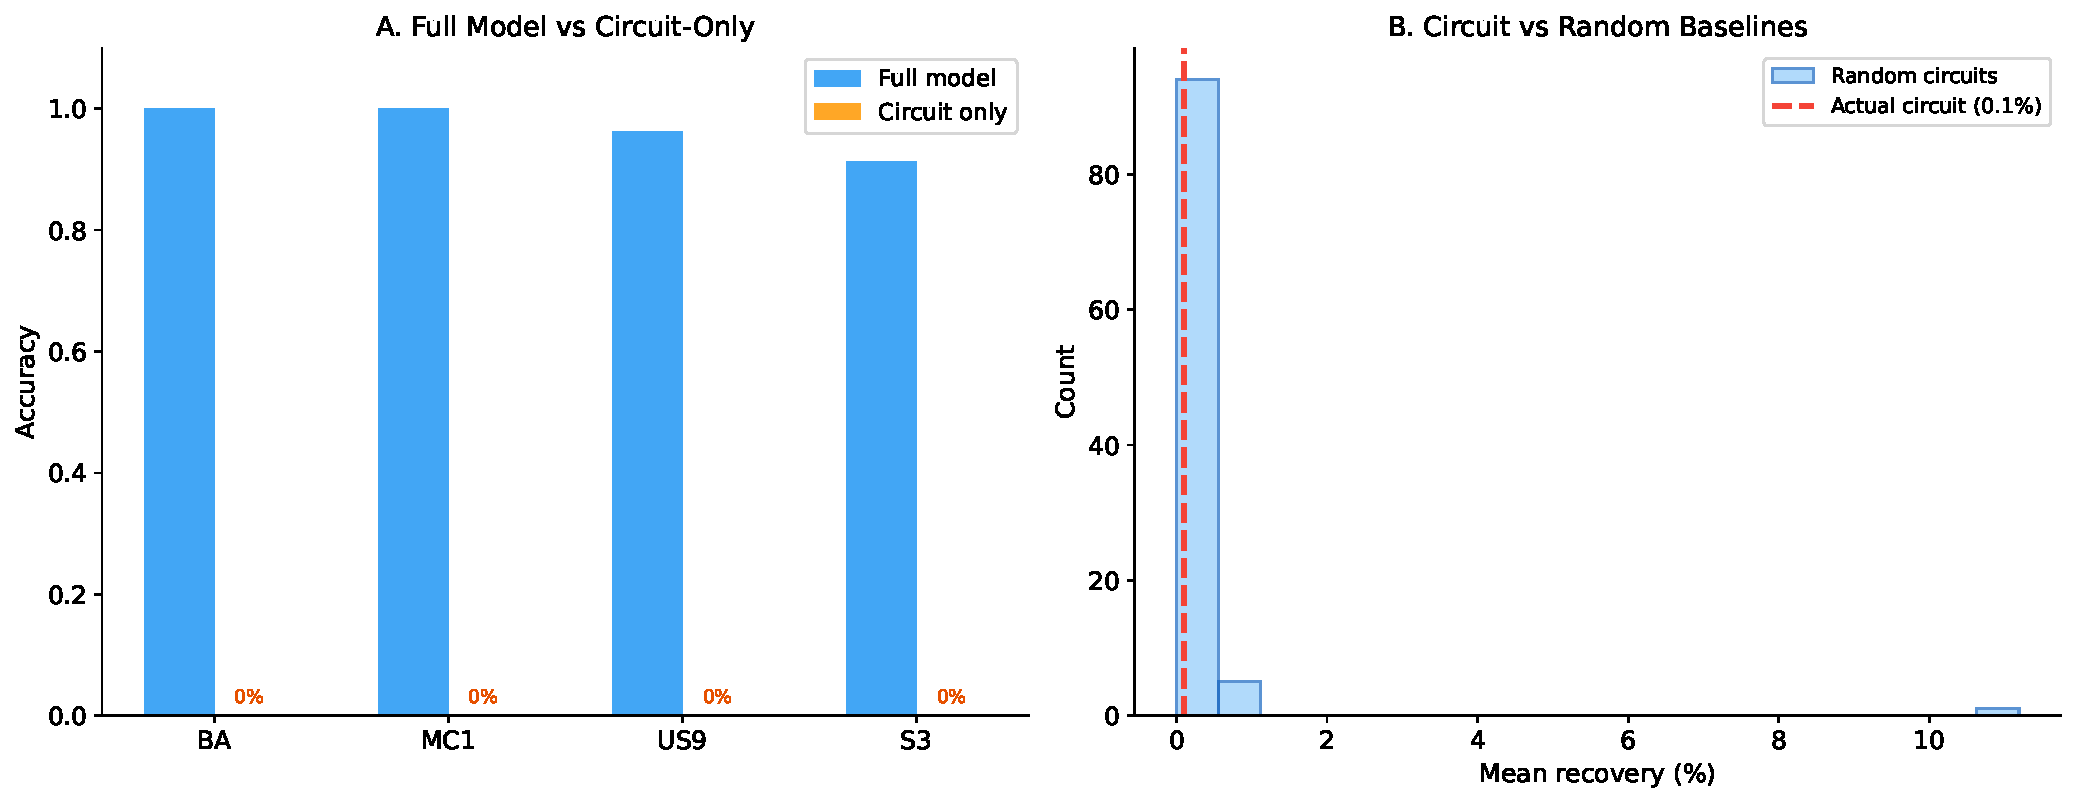
\includegraphics[width=\columnwidth]{figures/fig6_sufficiency.pdf}
\caption{Sufficiency testing. \textbf{A:} Circuit-only accuracy is near zero for all categories. \textbf{B:} The actual circuit's recovery is not significantly different from random circuits of equal size, because any 50\% subset of an 8-component model destroys too much shared infrastructure.}
\label{fig:sufficiency}
\end{figure}

\subsection{Compensatory Paths}

The assignment requires checking for paths that participate in carry propagation but were not detected in the initial sweep.
If compensatory circuits exist, single-component ablation may understate the true importance of the primary circuit.

After ablating the primary circuit heads (L0H1, L0H2), I re-measured IE for all non-circuit heads on Type~A ones pairs.
Three heads showed dramatic IE increases:
L0H0 rose from $-0.0001$ to $0.86$ (previously inactive, now strongly compensating);
L1H1 from $0.003$ to $0.50$;
L1H0 from $-0.008$ to $0.38$.

I call these active compensatory paths --- heads outside the primary circuit that partially take over when the circuit is knocked out.
The model's small size forces components into dual roles, so partial redundancy is expected. But the compensation is incomplete --- overall carry accuracy still collapses when the primary circuit is removed.

\subsection{Minimality}

Because the circuit's sufficiency recovery is only 0.1\%, removing any single component from the circuit does not meaningfully change the (already near-zero) circuit-only recovery.
Formally, all components appear ``redundant'' under this metric.
This is meaningless given 0.1\% sufficiency --- there is no baseline to degrade from. The necessity results already show L0H1 and L0H2 are individually essential.
A meaningful minimality test requires a circuit with sufficient recovery to measure degradation when components are removed.
With a larger model where the carry circuit achieves 80\%+ sufficiency, removing each component and measuring the recovery drop would directly test whether each is contributing unique information.

\section{Discussion}
\label{sec:discussion}

\paragraph{Main finding.}
Carry propagation in this model is partially localized. L0H1 and L0H2 are clearly necessary for carry --- ablating either one is devastating. But the circuit cannot run on its own; it depends on the base-addition infrastructure that the other components provide.
Two reference points from the literature:

\begin{itemize}
\item Quirke \& Barez~\cite{quirke2024understanding} found fully modular carry circuits in 2-layer models for 5-digit addition, with staircase attention patterns and high sufficiency.
\item Nikankin et al.~\cite{nikankin2024arithmetic} found that LLMs use a ``bag of heuristics'' with no coherent carry algorithm.
\end{itemize}

The model is small enough that components must serve multiple roles --- a 398K-parameter model with 6 attention heads cannot dedicate half of them to carry without starving base addition. The weak sufficiency is probably a capacity effect, not a fundamental property of how transformers solve arithmetic.

\paragraph{Absence of staircase patterns.}
Quirke \& Barez reported staircase attention in 5-digit models.
My 3-digit model shows no such pattern (Section~\ref{sec:attention}).
Staircase attention may only emerge when sequences are long enough that rigid positional routing is worth the specialization cost. Three digits might not cross that threshold.

\paragraph{The S3 failure mode.}
The model achieves only 91.3\% on full cascades.
The circuit results explain this: hundreds-carry computation is more distributed (max IE ${\approx}0.33$ vs.\ ${\approx}1.0$ for ones/tens), meaning no single head cleanly handles the final stage of a 3-position cascade.
The failures concentrate in the hundreds digit (92.5\% accuracy), exactly where the cascade must propagate furthest.

\paragraph{Connections to prior homework.}
Same thing happened in earlier assignments --- baselines that should help on CartPole turned out irrelevant (HW1), and GRPO could not bootstrap from a collapsed policy (HW2). Here, the ``obvious'' prediction that carry heads form a self-contained module also turned out wrong.

\section{Conclusion}
\label{sec:conclusion}

The L0H1 ablation result is the headline: one head removed, carry accuracy drops from 91\% to 0.4\%, non-carry stays at 99.7\%. That is a clean localization signal. But the circuit cannot stand alone --- it reads digit-pair sums computed by L0-MLP and other heads that also handle non-carry addition. Carry is a modifying overlay, not a standalone module.

The gap between this and Quirke \& Barez's fully modular circuits is probably a capacity effect. A 398K-parameter model with 6 attention heads cannot dedicate half of them to carry without starving everything else. With a 4-layer, 4-head model, I would expect the carry circuit to separate more cleanly --- and re-running the patching sweep on that model would test this directly.

\bibliographystyle{plainnat}
\bibliography{references}

\end{document}
